\begin{center}
     \Large{4. Data Structures and Memory Management}
\end{center}

\begin{center}
     \textbf{Data Structure Classification}
\end{center}
\begin{center}
    \begin{tabular}{ p{0.4\linewidth} p{0.5\linewidth} }
    \hline
    \textbf{Primitive} data fits into a memory location and is passed by value.
    & \textbf{Reference} data points to an address where the memory is stored. \\
    \rowcolor{yellow}
    \textbf{Scalar} data has only 1 value. & \textbf{Compound} data is composed of multiple elements. \\
    \textbf{Native} type are provided by the core language definition. & \textbf{Derived} types are implemented using other types. \\
    \rowcolor{yellow}
    \textbf{Random Access} data structures have O(1) access time and are usually 1 homogeneous structure.
    & \textbf{Recursive} data structures are constructed with smaller segments and have >O(1) access time. \\
    \textbf{Vectors} are re-sizeable and provide random access. & \textbf{Array} fixed-sized and provide random access. \\
    \hline
    \end{tabular}
\end{center}

\begin{center}
     \textbf{Modes of Use}
\end{center}
\begin{itemize}
    \item \textbf{Pass by Value} copies the value into the new memory location. \textbf{Pass by Reference} passes the reference to the data by value, copies the pointer to the data into the new memory location.
    \item \textbf{Mutability} determines if a data structure can be destructively modified after creation. \textbf{Constancy} determines if a variable can be reassigned another data after declaration.
\end{itemize}

\begin{center}
     \textbf{Allocation Types}
\end{center}
\begin{itemize}
    \item \textbf{Static Allocation} allocates memory at compile time. Runtime allocation like dynamically sized data and recursive functions are not possible. 
    \item \textbf{Stack Allocation} allows runtime memory allocation but requires data size to be known at compile time. Stack grows and shrinks by fixed amount determined at compile time for each function call. Stack is LIFO and thus chronologically ordered.
    \item \textbf{Heap Allocation} allocates and deallocates at run time in any order. Results in complex pointer structures which requires more complex memory management. 
\end{itemize}

\begin{center}
    \textbf{Heap Memory Model}
\end{center}
A heap is a directed graph references. Each node is a data structure and the edges are references between the data structures. A node can also point to a primitive. Mutators on the graph are either \code{createNode} or \code{updateEdge}.
\begin{center}
    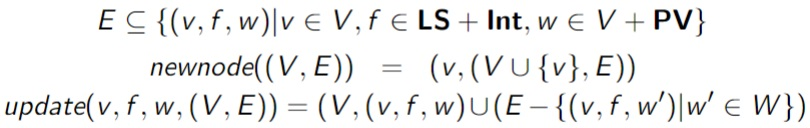
\includegraphics[scale=0.5]{images/heap model.jpg}
\end{center}

\begin{center}
    \textbf{Heap Selectors}
\end{center}
\begin{center}
    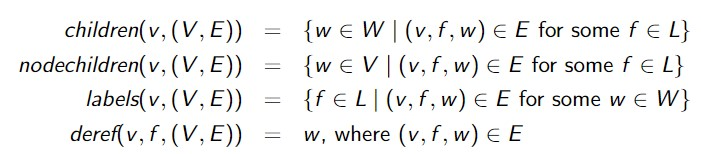
\includegraphics[scale=0.6]{images/heap selectors.jpg}
\end{center}

\begin{center}
    \textbf{Heap Management Techniques}
\end{center}
\begin{itemize}
    \item \textbf{Reference Counting} identifies and removes all nodes with no incoming edges. Each data structure can be deallocated without waiting for a global garbage collector(incrementality) and the memory can be immediately reused. This also preserves locality for caching purposes. However, it imposes a runtime overhead and cannot reclaim memory with cyclic references.
    \item \textbf{Mark \& Sweep} marks every node that is reachable from the root node and then deallocates all unreachable nodes. \\
    \begin{center}\begin{tabular}{ c c }
        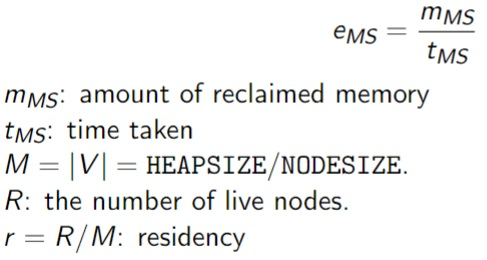
\includegraphics[scale=0.5]{images/mark n sweep 1.jpg} & 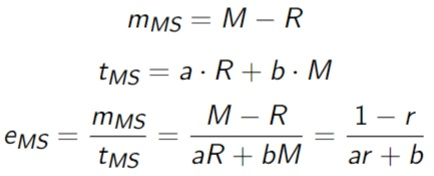
\includegraphics[scale=0.5]{images/mark n sweep 2.jpg} 
    \end{tabular}\end{center}
    \item \textbf{Copy Garbage Collection} partitions the heap into 2, with only one side being active at once. Once the active side fills up, copy all the live memory into the other side, set it as active, and deallocate all memory in the old active side.
    \begin{center}
        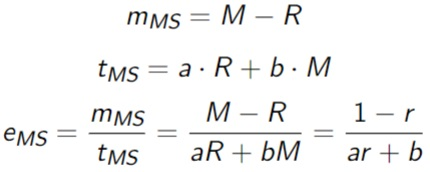
\includegraphics[scale=0.5]{images/copy garbage collection.jpg}
    \end{center}

    \item Copy Garbage Collection is more at low residency than Mark and Sweep but this flips as residency increases. At half residency, Copy Garbage Collection can no longer free any memory and thus has 0 efficiency.
    \begin{center}
        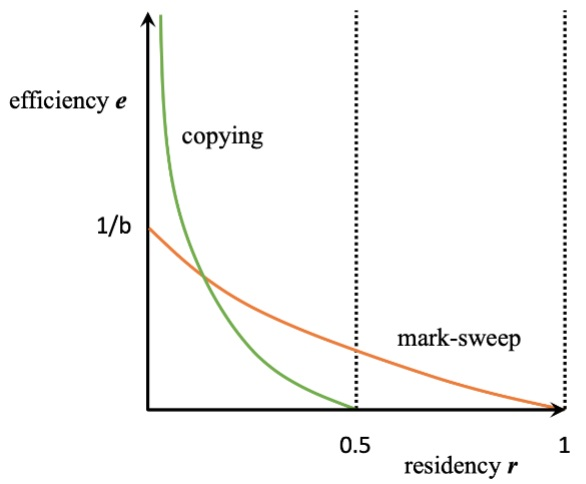
\includegraphics[scale=0.5]{images/efficiency graph.jpg}
    \end{center}
\end{itemize}